\section{Dataset Construction}
\label{sec:dataset}

OenoBench is constructed by an LLM-driven pipeline (Figure~\ref{fig:pipeline})
in two stages: (1) a \emph{fact-collection} stage that builds a corpus of
atomic, provenance-tagged statements from authoritative sources, and (2) a
\emph{question-generation} stage that converts those facts into benchmark
questions using five complementary strategies and five generator models.
The pipeline is designed around a single methodological commitment: large
language models are used as \emph{rephrasers and auditors}, never as the
source of truth. Every fact in the corpus traces to a URL with a tier-of-authority
label, every question is anchored in one or more such facts, and every
question is scored by a nine-agent automated audit (Section~\ref{sec:audit})
before release.

\begin{figure}[t]
  \centering
  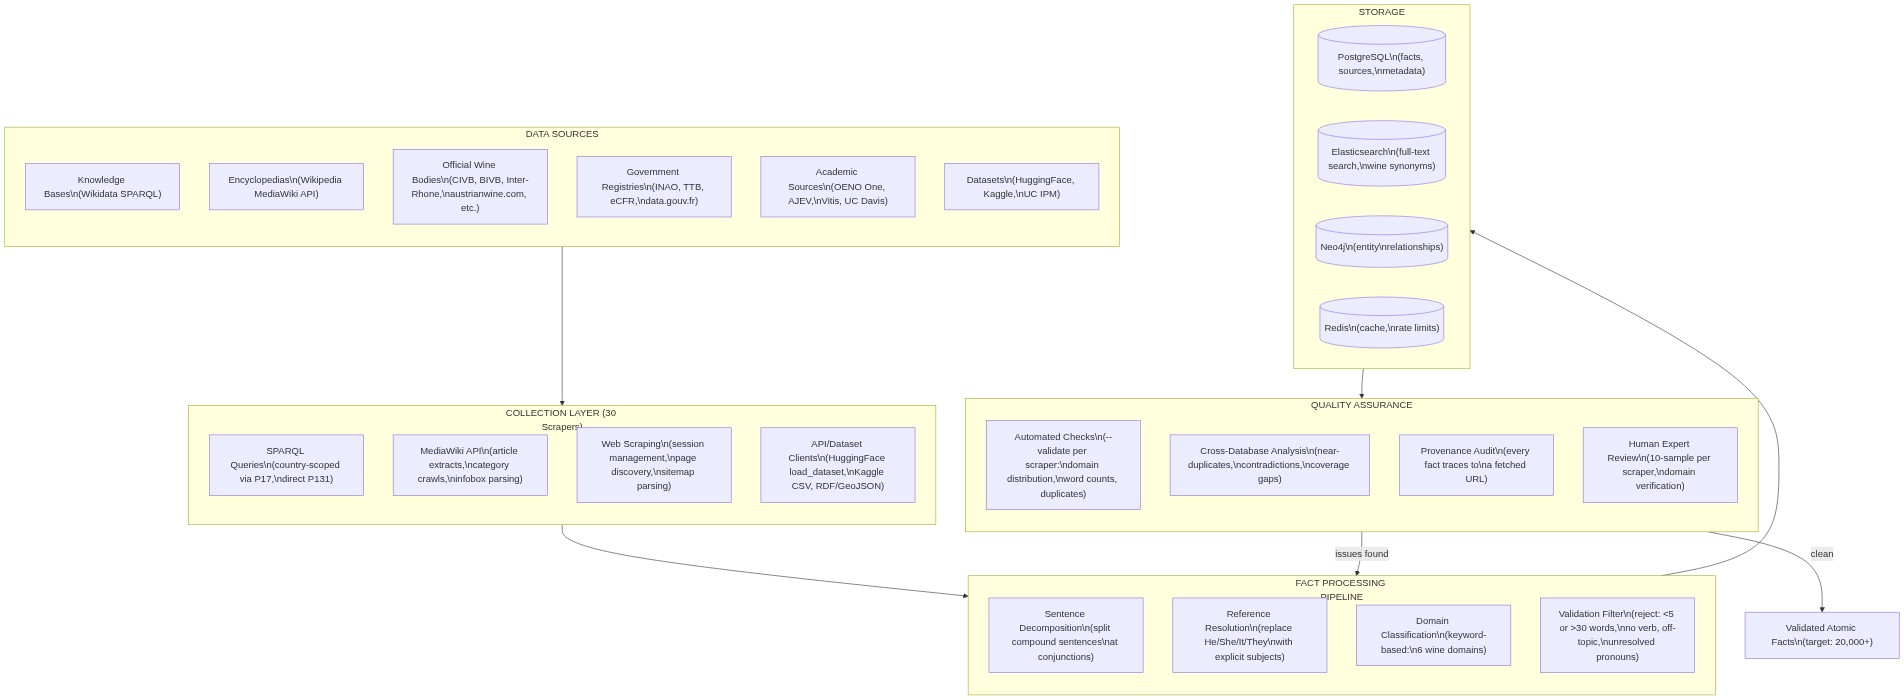
\includegraphics[width=0.95\linewidth]{figures/diagram_pipeline.png}
  \caption{End-to-end pipeline. Authoritative sources (top) are scraped
    by 35 source-specific extractors that share an atomic-fact decomposition
    and validation pass. Generated questions are gated by a closed-book
    pre-screen and a nine-agent audit before being tagged for release.}
  \label{fig:pipeline}
\end{figure}

\subsection{Domain taxonomy}
We organise wine knowledge into six \emph{domain pillars}, chosen to align
with the WSET Level~3 and Diploma syllabi:
(i) \textbf{wine regions} (appellations, classifications, geography,
climate, soils);
(ii) \textbf{grape varieties} (ampelography, parentage, regional
distribution, sensory profile);
(iii) \textbf{viticulture} (vineyard practice, training systems, pests
and diseases, vintage effects);
(iv) \textbf{winemaking} (vinification choices, fermentation, ageing,
faults);
(v) \textbf{producers} (estates, n\'egociants, co-operatives, key
houses); and
(vi) \textbf{wine business} (markets, regulation, distribution,
economics).
Each domain has a separate target share informed by syllabus weighting
and source availability; the realised distribution is reported in
Table~\ref{tab:facts}.

\subsection{Source tiering and provenance integrity}
\label{sec:sources}
Every fact is tagged with one of three source tiers, mirroring
evidence-based-medicine practice:
\begin{itemize}\itemsep -1pt
  \item \textbf{Tier~1 (official, 19.6\%):} government registries and
    inter-governmental bodies (INAO, OIV, TTB, regional consortia, the
    UC Davis AVA database).
  \item \textbf{Tier~2 (authoritative, 76.6\%):} Wikipedia (34.3\% of
    facts), Wikidata SPARQL (31.0\%), wine-body and consortium websites,
    peer-reviewed journals (\emph{OENO One}, \emph{Vitis}, \emph{Australian
    Journal of Grape and Wine Research}).
  \item \textbf{Tier~3 (reliable, 3.8\%):} curated open datasets on
    HuggingFace and Kaggle, secondary reference databases.
\end{itemize}

A 2026-04 internal audit identified 19 of an earlier 35-scraper set
whose ``scraped'' facts were in fact hard-coded LLM-generated content.
All 19 were rebuilt against live sources, the corpus was purged of
24{,}563~$\rightarrow$~16{,}702 facts and rebuilt to the current
38{,}104, and the entire fact corpus reported here passes a per-source
URL trace check. We document this rebuild because we believe that
\textbf{provenance auditing should be a first-class step in any
LLM-built benchmark}: model-generated content masquerading as scraped
data is a contamination vector that conventional dataset documentation
does not detect, and the fix is mechanical only if scraper code is
released alongside the data.

\begin{table}[t]
  \centering
  \caption{Atomic-fact corpus: 38{,}104 facts from 35 scrapers, six
    domain pillars, three source tiers.}
  \label{tab:facts}
  \small
  \begin{tabular}{lrrrr}
    \toprule
    Domain pillar & Facts & Share & Tier~1 & Tier~2/3 \\
    \midrule
    Wine regions     & 18{,}943 & 49.7\% & 23.4\% & 76.6\% \\
    Producers        &  6{,}215 & 16.3\% &  9.1\% & 90.9\% \\
    Grape varieties  &  5{,}959 & 15.6\% & 18.8\% & 81.2\% \\
    Viticulture      &  3{,}635 &  9.5\% & 12.0\% & 88.0\% \\
    Wine business    &  1{,}985 &  5.2\% & 31.4\% & 68.6\% \\
    Winemaking       &  1{,}367 &  3.6\% & 16.7\% & 83.3\% \\
    \midrule
    \textbf{Total}   & \textbf{38{,}104} & \textbf{100.0\%} &
                       \textbf{19.6\%} & \textbf{80.4\%} \\
    \bottomrule
  \end{tabular}
\end{table}

\subsection{Atomic fact extraction}
\label{sec:extraction}
Source pages are decomposed into atomic facts by a five-stage pipeline
(Figure~\ref{fig:fact_processing}): (1) sentence splitting at
conjunctions and clause boundaries, (2) reference resolution (pronouns
and demonstratives are replaced with their entity referents from article
context), (3) domain classification into one of the six pillars, (4) a
length-and-predicate validator that rejects facts shorter than five
words, longer than fifty words, missing a verb, or carrying dangling
references, and (5) an on-topic filter parameterised by region-specific
keyword sets to prevent cross-contamination (e.g.\ Austrian content
appearing in a Bordeaux scraper). Wikidata SPARQL queries use direct
country relations (\texttt{P17}) rather than transitive administrative
parents (\texttt{P131*}); the latter caused severe cross-region leakage
in early scrapers and is documented as a cautionary case in
Appendix~\ref{app:methodology}.

\begin{figure}[t]
  \centering
  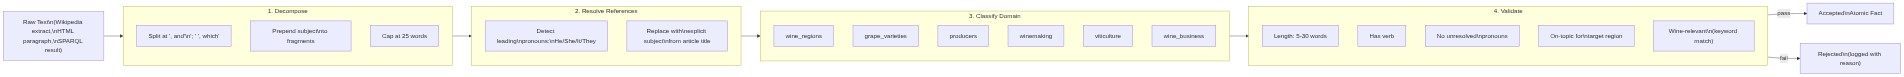
\includegraphics[width=0.85\linewidth]{figures/diagram_fact_processing.png}
  \caption{Atomic-fact extraction pipeline. Inputs are heterogeneous
    (HTML pages, RDF graphs, SPARQL responses, CSV dumps); outputs are
    uniform single-assertion sentences with entity tags, domain label,
    source URL and tier.}
  \label{fig:fact_processing}
\end{figure}

Facts are required to be (a) \emph{atomic}, one assertion per sentence;
(b) \emph{entity-tagged}, with subject and object linked to canonical
IDs in the wine knowledge graph; and (c) \emph{source-faithful}, a
paraphrase of the original, never a verbatim copy. This last constraint
is enforced both at extraction time and at audit time
(Section~\ref{sec:audit}, agent A3).

\subsection{Question generation: five strategies, five models}
\label{sec:generation}
A single-strategy, single-model benchmark inherits the blind-spots of
its pipeline. We mitigate this by combining \emph{five strategies} and
\emph{five generator models}, with per-strategy and per-model quotas
enforced by an orchestrator that resumes safely across runs. Strategies
are:
\begin{itemize}\itemsep -1pt
  \item \textbf{Fact-to-question (58.4\%, 1{,}909 questions):} the LLM
    rewrites a single verified fact as a multiple-choice question;
    preserves grounding but tends toward recall.
  \item \textbf{Distractor mining (12.4\%, 405):} confusable-entity
    sampling produces wrong answers that share the right answer's
    category and dimension, raising plausibility and forcing
    fine-grained discrimination.
  \item \textbf{Template (11.9\%, 389):} forty-five deterministic
    parameterised templates across the six pillars; pure entity
    substitution, zero LLM creativity --- a baseline against which
    neural generation is measured.
  \item \textbf{Scenario synthesis (9.8\%, 319):} coherent fact clusters
    are converted into applied multi-fact reasoning prompts (e.g.\ a
    sommelier service decision, a winemaker blending decision, a
    viticulturist vintage call). Domain-specific scenario types prevent
    persona-content mismatch.
  \item \textbf{Comparative (7.5\%, 244):} entity-affinity scoring pairs
    related entities (e.g.\ two Burgundy premiers crus, two Rh\^one
    grapes) and asks ``which differs in X'' or ``what do both share''.
\end{itemize}

The five generator models are Claude Opus 4.7, GPT-5, Gemini 2.5 Pro,
Llama 3.1 405B, and Qwen 3.5 235B, each accessed through a unified
OpenRouter client with consistent temperature and top-$p$. Generator
distribution across the corpus is approximately Qwen 20\%, Llama 19\%,
Claude 19\%, ChatGPT 17\%, Gemini 13\%, deterministic templates 12\%.

\paragraph{Closed-book gate.} Questions targeting difficulty levels~1
and~2 are passed through a \emph{closed-book pre-screen} before
admission: a separate LLM (Claude Sonnet for L1, Opus for L2) attempts
the question with no source fact in context, and questions it answers
correctly are tagged \texttt{closed\_book\_solvable} and reserved into a
quota (target $<$25\%). Difficulty levels~3 and~4 skip the gate by
protocol, since high-difficulty items are expected to be answerable only
with the supporting fact. The audit's B2 agent
(Section~\ref{sec:audit}) re-runs this check at corpus scale on a panel
of three judges; we discuss its calibration against humans and the
implications for the eval contrast in Section~\ref{sec:eval-cb}.

\subsection{Final corpus: \texttt{release\_v1.2}}
\label{sec:release}
After generation, audit, and post-eval review, the released corpus
\texttt{release\_v1.2} contains \textbf{3{,}266 questions}. The
distribution along three axes is:

\begin{table}[h]
  \centering
  \caption{Composition of the released corpus.}
  \label{tab:corpus}
  \small
  \begin{tabular}{lrrlrr}
    \toprule
    Domain & N & \% & Difficulty & N & \% \\
    \midrule
    Wine regions     & 1{,}108 & 33.9\% & L1 (entry)        & 694   & 21.2\% \\
    Grape varieties  & 766     & 23.5\% & L2 (intermediate) & 894   & 27.4\% \\
    Producers        & 515     & 15.8\% & L3 (advanced)     & 678   & 20.8\% \\
    Viticulture      & 502     & 15.4\% & L4 (expert)       & 1{,}001 & 30.6\% \\
    Wine business    & 250     &  7.7\% &                   &       &       \\
    Winemaking       & 187     &  5.7\% &                   &       &       \\
    \midrule
    \textbf{Total}   & \textbf{3{,}266} & \textbf{100\%}
                     & \textbf{Total}   & \textbf{3{,}266} & \textbf{100\%} \\
    \bottomrule
  \end{tabular}
\end{table}

The corpus underwent two post-generation passes: a 9-agent automated
audit (Section~\ref{sec:audit}) that dropped 341 questions and re-labelled
the difficulty of 1{,}259, and a post-evaluation review of 97 items that
were answered incorrectly by all 16 evaluation configurations
(Section~\ref{sec:eval}, Appendix~\ref{app:eval}), of which 54 were
removed as defects, 9 were dropped after a borderline-review pass, and
the remainder retained as legitimately hard items.
